\documentclass[11pt, oneside]{article}
 
% PKG : police du rapport 
\usepackage[sfdefault]{roboto} 
\usepackage[T1]{fontenc}
\usepackage[utf8]{inputenc}


%%%%%%%%%%%%%%%%%%%%%%%%%%%%%%%%%%%%%%%%%%%%%%%%%%%%%%%%%%%%%%%%%%%%%%%%
%%%%%%%%%%%%%%%%%%%%%%%%%%% ZONE A CHANGER %%%%%%%%%%%%%%%%%%%%%%%%%%%%%
%%%%%%%%%%%%%%%%%%%%%%%%%%%%%%%%%%%%%%%%%%%%%%%%%%%%%%%%%%%%%%%%%%%%%%%%

\newcommand{\type}{30/05/2018}	% Date
			 
%%%%%%%%%%%%%%%%%%%%%%%%%%%%%%%%%%%%%%%%%%%%%%%%%%%%%%%%%%%%%%%%%%%%%%%%
%%%%%%%%%%%%%%%%%%%%%%%%%% NE PAS Y TOUCHER %%%%%%%%%%%%%%%%%%%%%%%%%%%%
%%%%%%%%%%%%%%%%%%%%%%%%%%%%%%%%%%%%%%%%%%%%%%%%%%%%%%%%%%%%%%%%%%%%%%%%
\newcommand{\titre}{Rapport final - PEE InMoov}

%Table des matière intéractif et URL
\usepackage{hyperref}
 
\usepackage[head=30pt,foot=30pt,top=3cm, bottom=3.5cm, outer=2cm, inner=2cm]{geometry}

% PKG : images
\usepackage{graphicx}

% PKG : couleur
\usepackage{xcolor}

% PKG : mise en page
\usepackage{lipsum}

% PKG : item 
\usepackage{enumitem}
\usepackage{pifont}

% PKG : position image avec H en parametre 
\usepackage{float}

% PKG : header et footer
\usepackage{lastpage} 
\usepackage{fancyhdr}
\pagestyle{fancy}

% PKG : pour avoir les dates en francais 
\usepackage[english,francais]{babel}

\usepackage{scrextend}

\usepackage{titlesec}
\newcommand{\sectionbreak}{\clearpage}


\fancypagestyle{style}{
\fancyhf{}
\lhead{
\includegraphics[width=5cm]{img_template/DaVinciBot_Banner.png}}
\chead{\color{gris} \textbf{\titre\\}}
\rhead{
\includegraphics[width=4cm]{img_template/Logo_InMoov.png}\vspace{0.1cm}}
\lfoot{ \type  }
\rfoot{Page \thepage\ sur \pageref{LastPage}}
}

% ---- COLOR ---- %
\definecolor{gris}{rgb}{0.36,0.36,0.36}
\definecolor{bleu}{rgb}{0.1137,0.4941,0.5921}
\definecolor{gristitle}{rgb}{0.95,0.95,0.95}

\hypersetup{%
  colorlinks = true,
  linkcolor  = black,
  urlcolor = gris 
}
 
\setlength{\parskip}{1em}
\renewcommand{\baselinestretch}{1.2}

%%%%%%%%%%%%%%%%%%%%%%%%%%%%%%%%%%%%%%%%%%%%%%%%%%%%%%%%%%%%%%%%%%%%%%%%%
%%%%%%%%%%%%%%%%%%%%%%%%%%%% PAGE DE GARDE %%%%%%%%%%%%%%%%%%%%%%%%%%%%%%
%%%%%%%%%%%%%%%%%%%%%%%%%%%%%%%%%%%%%%%%%%%%%%%%%%%%%%%%%%%%%%%%%%%%%%%%%

\begin{document}
\pagestyle{style}

\begin{center}
\begin{minipage}{0.75\linewidth}
\begin{center}
\centering
   
\vspace{2cm}
\colorbox{gristitle}{
\begin{minipage}{\textwidth}
    \begin{center}
    	\vspace{0.5cm}
    	%% Titre et sous titre 
    	{\color{bleu} \uppercase{\Huge {\titre}}}
    	\vspace{0.25cm}\linebreak
		\par \color{gris} {\Large \type}	
	\end{center}    
\end{minipage}    
}

\vspace{1cm}
\begin{center}
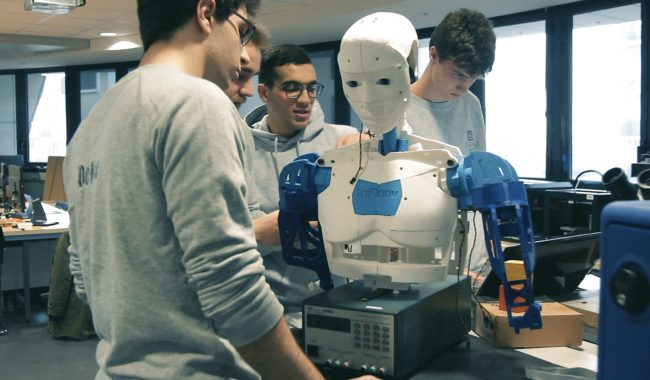
\includegraphics[width=14cm]{inmoov-robot.jpg}
\end{center}

\vspace{0.5cm}
% Description de Davincibot
\color{bleu} {\Large Participants au PEE InMoov  : \par}
\end{center}

\begin{itemize}
\item[•] Corentin LEMAITRE - ESILV - 4ème année - spécialisation IBO
\item[•] Hugo POUSSEUR - ESILV - 4ème année - spécialisation IBO
\item[•] Rabah HOUAOUI - ESILV - 4ème année - spécialisation IBO
\item[•] Brice PARILUSYAN - ESILV - 3ème année
\item[•] Nicolas FONTAINE - ESILV - 3ème année
\end{itemize}

\end{minipage}
\end{center}

\newpage


%%%%%%%%%%%%%%%%%%%%%%%%%%%%%%%%%%%%%%%%%%%%%%%%%%%%%%%%%%%%%%%%%%%%%%%%%
%%%%%%%%%%%%%%%%%%%%%%%%%%%%%%%% CONTENU %%%%%%%%%%%%%%%%%%%%%%%%%%%%%%%%
%%%%%%%%%%%%%%%%%%%%%%%%%%%%%%%%%%%%%%%%%%%%%%%%%%%%%%%%%%%%%%%%%%%%%%%%%

\tableofcontents

\section{Introduction}
\vspace{0.5cm}


\section{Description du projet}
Le projet consiste en la construction du robot humanoïde à taille humaine :InMoov.
		
Ce robot possède deux caractéristiques particulièrement intéressantes. Il est entièrement imprimable en 3D sur des imprimantes 3D classique. De plus c'est un robot OpenSOurce, ce qui signifie que tout est public réutilisable et modifiable. Nous avons donc accès à toutes les modélisations du robot, de tutoriels, de code informatique...

Notre objectif dans ce PEE est de construire le robot afin qu'il puissent être utilisé par la suite par l'association DaVinciBot pour, par exemple :
	\begin{itemize}
		\item Servir à la communication de l'association et du Pôle universitaire Léonard De Vinci lors d'évènements tels que les JPO.
		\item Devenir une plateforme d'innovation Pour les différents projets que les membres de l'association souhaiterons entreprendre avec. Sa structure imprimable en 3D le rend modulaire et donc amène d'accueillir de futur améliorations et extensions, le tout à moindre coût.
		\item L'améliorer pour ensuite partagé nos avancées avec la communauté InMoov (trois PI² ont déjà été créés pour améliorer le robot).
	\end{itemize}
	
	
\section{Organisation du projet}	 

Les impressions des pièces du robot étant le fil rouge du projet pendant la première phase du projet, optimiser cette partie était primordiale. Nous avons donc établi quelques règles :
	\begin{itemize}
	\item Nous avons assigné à chacun un jour de la semaine. Pendant cette journée la personne doit imprimer le plus de pièce possible sur les imprimantes 3D afin de faire avancer au plus vite le projet.
	\item Afin de savoir les pièces qui ont été imprimé et celles qui restaient à imprimer, un fichier Excel partagé a été créé. Ce fichier regroupe toutes les données sur les pièces imprimées et à imprimer et était mis à jour à chaque nouvelle impression.
	\item Toutes les pièces devant être imprimé étaient stockées sur une clé USB avec leurs paramètres d'impression déjà attribués, accélérant ainsi le processus d'impression.
	\item Lorsque suffisamment de pièce était imprimé, nous nous réunissions alors au plus vite afin de construire la partie en question.
	\end{itemize}

Une fois les parties impression et construction réalisées, nous devions motoriser le robot. Pour cela, nous avons dû créer nos carte électroniques afin de partager l'alimentation dans les différents servomoteurs. Ensuite, nous avons dû programmer ces servomoteurs avec un logiciel dédié : MyRobotLab.

\vspace{1cm}
\section{Bilan  / apprentissage}
\vspace{0.5cm}
\begin{description}
\item[Impressions 3D :] Nous avons appris à utiliser une imprimante 3D mais surtout à l'entretenir et régler les différents problèmes qui lui surviennent au fil des mois.
\item[L'assemblage du robot :] Pour Construire le robot, nous avons dû poncer des pièces, démonter des objets pour en récupérer des composants(caméra, moteur...) et enfin assembler les différentes pièces. Pour faire cela nous avons appris à utiliser les outils de construction et des fers à souder.
\item[L'électronique :] Nous devons, pour construire ce robot, utiliser nos compétences d'électronique vue en première et deuxième année à l'ESILV pour connecter tous les capteurs et moteurs du robot.
\item[Programmation :] Pour rendre le robot plus vivant, il faut coder les moteurs du robot. Nous devons donc utiliser nos compétences de programmation.
\end{description}

\section{Contributions individuelles}
\subsection{Corentin LEMAITRE}
\vspace{0.5cm}

Dans ce PEE, je m’occupe d’imprimer des pièces le mercredi. Je lance les premières impressions à 8h30 et les dernières en fin de journée. Avant ce projet, je ne savais pas du tout utiliser une imprimante 3D. Grâce aux nombreuses impressions que l'on doit effectuer, j'ai appris à transformer des fichiers de conception de pièces 3D (les STL pour STereo-Lithography)  au format exigé par nos imprimantes, et ensuite, à suivre toutes les étapes mécaniques et informatiques pour veiller au bon déroulement des impressions.\\
Je me suis également occupé de créer le fichier Excel permettant le suivi de chaque impression. En effet, sur ce fichier est inscrit toutes les pièces nécessaires à la construction d'InMoov. Il permet de savoir où on se trouve dans l'avancement des impressions mais également de prévoir quelles impressions sont encore à effectuer et avec quels paramètres. Enfin, ce fichier nous aide à regrouper des statistiques de construction sur le robot comme, par exemple, le temps total des impressions ou la quantité de fil utilisé pour chaque impression. La création de ce fichier m'a permis de compléter mes connaissances sur Excel et nous sert également à planifier de manière assidue les impressions du projet. 
\paragraph{}
Comme chacun des membres du projet, j'ai appris la partie mécanique (ponçage, percage et montage) au fil de l'avancement du projet. Malgré quelques tutoriels à notre disposition sur internet, il a souvent été difficile de savoir comment monter des pièces et parvenir à la même réalisation que le robot officiel. Il a donc fallu réfléchir par nous-mêmes et parfois se renseigner auprès de la communauté InMoov pour franchir des étapes. \\
Nous faisons partie d’une équipe très motivée ou une ambiance très amicale règne constamment ce qui facilite considérablement le travail en groupe. Nous avons tous déjà travaillé ensemble sur plusieurs projets auparavant donc le fait de se connaitre est un véritable atout dans l'organisation du PEE. De plus, nous avons pris pour habitude de faire des réunions régulières permettant de régler les problèmes urgents rapidement pour ne pas perturber l'avancement du projet.


\subsection{Hugo POUSSEUR}

\vspace{0.5cm}

Dans ce PEE, je m'occupe d'imprimer des pièces le mardi et le samedi. Je lance les premières impressions à 8h30 et les dernières en fin de journée.  Ce qui m'a permis d'accroitre mes connaissances sur la gestion d'imprimante 3D, notamment sur les impressions en ABS (et de me sensibilisé sur la partie sécurité de l'impression de tels matériaux).\\ 
Avant de monter les composants électroniques sur le robot(servo moteur) j'ai dû les tester au préalable pour vérifier leur bon fonctionnement afin d'éviter de devoir tout démonter par la suite lors des tests réels.\\
 Ce projet m'a permis de découvrir des façons ingénieuses pour transmettre des mouvements, notamment des techniques permettant de convertir une rotation en translation.


\subsection{Rabah HOUAOUI}
\vspace{0.5cm}

Dans ce PEE, je m'occupe d'imprimer des pièces le lundi. Je lance les premières impressions à 8h30 et les dernières en fin de journée. J'étais également en charge du ponçage des pièces du robot. De plus j'ai également participé à la construction des yeux et à l'assemblage du torse du robot.  \\
J'ai également améliorer mes compétences techniques car le ponçage des pièces du robot est un travail de précision, il fallait donc être extrêmement attentif et veiller à ne pas déformer voir casser la pièce. Il en est de même pour l'assemblage du robot qui nécessite attention et minutions surtout pour la partie des yeux. J'ai aussi beaucoup appris à travers ce projet à comprendre l'utilisation et le fonctionnement des imprimantes 3D. 
\paragraph{} Au sein de l'équipe règne une atmosphère très agréable ce qui permet une meilleure collaboration avec les membres de l'équipe tout en étant performant dans la réalisation du projet. \\
Pour l'organisation, nous avons décidé de mettre en place un planning dans lequel pour chaque jour donné une personne de l'équipe est en charge des impressions des pièces 3D. De plus les pièces de notre robots étant nombreuses, nous avons mis en place un fichier Excel les répertoriant toutes afin d'avoir un suivi sur le travail réalisé et celui qu'il nous reste à faire \\
Ce projet est très enrichissant du point de vue technique car il m'a permis d'améliorer mon savoir-faire mais également mon savoir-être. Ainsi je pense que les compétences acquises avec ce projet vont m'être très utile dans mon avenir professionnel. 

\subsection{Brice PARILUSYAN}
\vspace{0.5cm}

Dans ce PEE, je m'occupe d'imprimer des pièces le jeudi et le samedi. Je lance les premières impressions à 8h30 et les dernières en fin de journée. J'ai participé à la construction de la tête ainsi que du torse de l'androïde. \\
J'ai aussi notamment appris à me servir des nouvelles imprimantes que nous avons reçu, les Raise3d. Je m'occupe de configurer les paramètres d'impressions des pièces avec le logiciel IdeaMaker. Ol me faut parfois adaptés les paramètres pour imprimer certaines pièces difficiles.\\
Ce projet me plaît énormément car entre parfaitement dans mon projet d'avenir.


\subsection{Nicolas FONTAINE}
\vspace{0.5cm}

Dans ce PEE, je m'occupe d'imprimer des pièces le vendredi. Je lance les premières impressions à 8h30 et les dernières en fin de journée.
De plus, j'ai appris à utiliser un fer à souder pour réaliser les circuits imprimés du robot. J'ai ensuite participer à l'assemblage de la tête et des épaules.
\newline
Pendant ce semestre, j'ai beaucoup appris sur l'utilisation et le fonctionnement des imprimantes 3D. Mais aussi sur les étapes de construction d'un tel robot.
\newline
Ce projet m'apporte beaucoup de compétences en robotique, un secteur qui m'intéresse énormément. 

\section{Conclusion}
\vspace{0.5cm}

Chacun de nous consacre beaucoup de temps pour ce PEE. De plus nous nous rassemblons souvent pour avancer ensemble ou réfléchir sur les prochaines actions à réalisées. Notre groupe est très bien organisé ce qui permet de bien avancer sur le projet malgré les retards en début de semestre dû à la livraison des imprimantes 3D.


\end{document}